\documentclass{article}

\usepackage[T2A]{fontenc}
\usepackage[utf8]{inputenc}
\usepackage[russian]{babel}
\parindent 0pt
\parskip 8pt
\usepackage{setspace}
\usepackage{amsmath}
\usepackage{amssymb}
\usepackage{amsfonts}
\usepackage[left=2.3cm, right=2.3cm, top=2.7cm, bottom=2.7cm, bindingoffset=0cm]{geometry}
\usepackage{latexsym}
\usepackage[unicode, pdftex]{hyperref}
\usepackage{xcolor}
\usepackage{graphicx}
\graphicspath{ {./images/} }

\onehalfspacing

\begin{document}

\tableofcontents

\newpage

\part{Определения}

	\newpage
	
	\section{Первообразная, неопределенный интеграл}
	
	\subsection{Первообразная}
	
		$f: \langle a, b \rangle \rightarrow \mathbb{R}$
	
		$F: \langle a, b \rangle \rightarrow \mathbb{R}$ ~--- первообразная $f$ на $\langle a, b \rangle$, если для любого $x \in \langle a, b \rangle$, $F$ ~--- дифференцируема в точке $x$, и $F'(x) = f(x)$.
	
		\underline{Пример}
	
		$f(x) = \sin{x} \Leftrightarrow F(x) = -\cos{x} + C$
	
	\subsection{Неопределенный интеграл}
	
		Неопределенным интегралом функции $f$ на $\langle a, b \rangle$ называют множество всех её первообразных.
		
		Обозначение: $\int{f}$, $\int{f(x) dx} = \left\{ F + C, C \in \mathbb{R} \right\}$, где $F$ ~--- любая первообразная.
		
		\newpage
		
		\section{Теорема о существовании первообразной}
		
			Пусть $f$ непрерывна на $\langle a, b \rangle \Rightarrow$ существует такая функция $F$ на $\langle a, b \rangle$, что $F' = f$.
			
			\textbf{Доказательство}
			
			В кредит
			
		\newpage
		
		\section{Таблица первообразных}
		
			\begin{enumerate}
			
				\item $f(x) = k$, $F(x) = kx$
				
				\item $f(x) = x^n$, $F(x) = \frac{x^{n + 1}}{n + 1}$
				
				\item $f(x) = \frac{1}{x}$, $F(x) = \ln |x|$
				
				\item $f(x) = e^x$, $F(x) = e^x$
				
				\item $f(x) = a^x$, $F(x) = \frac{a^x}{\ln a}$
				
				\item $f(x) = \sin{x}$, $F(x) = -\cos{x}$
				
				\item $f(x) = \cos{x}$, $F(x) = \sin{x}$
				
				\item $f(x) = \frac{1}{\sin^2{x}}$, $F(x) = -\ctg{x}$
				
				\item $f(x) = \frac{1}{\cos^2{x}}$, $F(x) = \tg{x}$
				
				\item $f(x) = \frac{1}{\sqrt{1 - x^2}}$, $F(x) = \arcsin{x}$
				
				\item $f(x) = \frac{1}{1 + x^2}$, $F(x) = \arctg{x}$
				
			\end{enumerate}
			
		\newpage
		
		\section{Равномерная непрерывность}
		
			Функция $f : \langle a, b \rangle \rightarrow \mathbb{R}$ равномерно непрерывна на $\langle a, b \rangle$, если:
			
			$\forall \varepsilon > 0$ $\exists \delta > 0$, $\forall x_0, x$ : $|x - x_0| < \delta$, $|f(x) - f(x_0)| < \varepsilon$
			
		\newpage
		
		\section{Площадь, аддитивность площади, ослабленная аддитивность}
		
			\subsection{Первое определение площади}
			
				Пусть $E$ ~--- множество всех ограниченных подмножество в $\mathbb{R}^2$ (или множество всех фигур).
			
				Тогда площадь ~--- это функция $\sigma$ : $E \rightarrow [0, +\infty)$ со свойствами:
			
				\begin{enumerate}
			
					\item аддитивность
				
						Если $A = A_1 \sqcup A_2 \Rightarrow \sigma(A) = \sigma(A_1) + \sigma(A_2)$
				
					\item нормировка
				
						$\sigma(\langle a, b \rangle \times \langle c, d \rangle) = (d - c)(b - a)$ 
		
				\end{enumerate}
			
				\underline{Замечание}
			
					Площадь монотонна, то есть если:	
			
					$A \subset B \Rightarrow \sigma(A) \leq \sigma(B)$
			
					$\sigma($вертикального отрезка$) = 0$
				
			\subsection{Второе определение площади}
			
				$\sigma : E \rightarrow [0, +\infty)$
				
				\begin{itemize}
				
					\item монотонна
					
					\item нормировка
					
					\item ослабленная аддитивность:
					
						$E = E_1 \cup E_2$, $E_1 \cap E_2$ ~--- вертикальный отрезок, $E_1$ и $E_2$ ~--- по разные стороны этого отрезка.
					
						$\sigma(E) = \sigma(E_1) + \sigma(E_2)$
						
				\end{itemize}
				
\newpage
	
\part{Теоремы}

	\newpage
	
	\section{Теорема Кантора о равномерной непрерывности}
	
		Пусть $f: X \rightarrow Y$ ~--- метрические пространства, $f$ непрерывна на $X$, $X$ ~--- компактно. Тогда $f$ ~--- равномерное непрерывно на $X$.
		
		\textbf{Доказательство (от противного)}
		
			Воспользуемся тем свойством, что если $X$ ~--- компактно, то $X$ и секвенциально компактно.
			
			Предположим противное:
			
			$\exists \varepsilon > 0$ \textcolor{gray}{$\delta = \frac{1}{n}$} $\exists x_n,  \widetilde{x_n}$: $\rho(x_n, \widetilde{x_n}) < \frac{1}{n}$ $\rho(f(x_n), f(\widetilde{x_n})) \geq \varepsilon$
			
			Тогда выберем сходящуюся подпоследовательность из $x_n$ $x_{n_k} \rightarrow a \in X$, $\widetilde{x_{n_k}} \rightarrow a \in X$.
			
			Тогда $f(x_{n_k}) \rightarrow f(a)$ и $f(\widetilde{x_{n_k}}) \rightarrow f(a)$, то
			
			$\rho(f(x_{n_k}), f(\widetilde{x_{n_k}})) \rightarrow 0$ (по неравенству треугольника)
			
			Что и противоречит изначальному условию.

	\newpage
	
	\section{Теорема Брауэра о неподвижной точке}
	
		Пусть $f: B(0, 1) \subset \mathbb{R}^m \rightarrow B(0, 1)$ ~--- непрерывное, тогда
		
		$\exists x_0 : f(x_0) = x_0$
		
		\textbf{Доказательство}
		
		\subsection{Игра ''Гекс''}
		
			Пусть есть поле $n \times m$, состоящее из правильных шестиугольников (гексов). Также два игрока на каждом своём ходу красят гексы в белый или чёрный цвет. Тогда для любой раскраски найдётся либо чёрная тропинка, соединяющая верхнюю и нижнюю часть поля, либо белая тропинка, соединяющая левую и правую часть поля.
			
			Доказывается от противного
		
			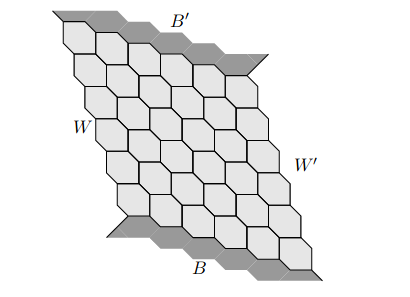
\includegraphics[scale=0.5]{HEX.png}
				
		\subsection{Сама теорема}
		
			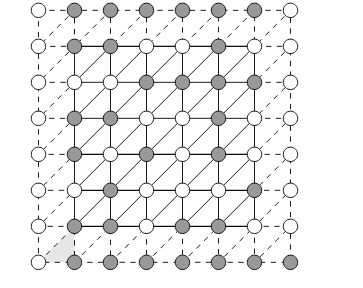
\includegraphics[scale=0.45]{NEWHEX.png}
		
			Теперь заменим гексы на обычную координатную плоскость, причём игра, по сути, останется такой же. Теперь перейдём к самой теореме.
			
			Шар с лёгкостью заменяется на обычный квадрат $[0, 1] \times [0, 1]$
			
			Пусть $f : [0, 1]^2 \rightarrow [0, 1]^2$ ~--- непрерывна. Тогда
			
			$\exists a \in [0, 1]^2$, $f(a) = a$
			
			$a \in [0, 1]^2$
			
			$a = (a_1, a_2)$
			
			$f(x) \in \mathbb{R}^2$
			
			$f(x) = (f(x)_1, f(x)_2)$
			
			\textbf{Доказательство}
			
				Пусть $\rho$ ~--- функция, заданная на $[0, 1]^2 \times [0, 1]^2$
				
				$\rho(x, y) = \max (|x_1 - y_1|, |x_2 - y_2|)$ ~--- непрерывна на $[0, 1]^2$
				
				$x_n \rightarrow a$
				
				$y_n \rightarrow b$
				
				$\rho(x_n, y_n) \rightarrow \rho(a, b)$
				
				Очевидно, что для любых $x, y: x \neq y \Rightarrow \rho(x, y) > 0$
				
				\underline{Теперь к самой теореме}
				
				Пусть для любого $x \in [0, 1]^2$ $f(x) \neq x$. Тогда $\rho(x, f(x)) > 0$, но $\rho$ непрерывно по $x$ и $[0, 1]^2$ ~--- компакт, значит по теореме Вейерштрасса существует такое $\varepsilon > 0$, что
				
				$\min\limits_{x \in [0, 1]^2} \rho(x, f(x)) = \varepsilon > 0$
				
				По теореме Кантора для этого $\varepsilon$ найдётся такая $\delta$ (будем считать, что $\sqrt{2} \delta < \varepsilon$), что
				
				$\forall x, \widehat{x} \in [0, 1]^2 : \| x - \widehat{x} \| < \delta \cdot \sqrt{2} \Rightarrow \| f(x) - f(\widehat{x}) \| < \varepsilon$
				
				Берём $\frac{1}{n} < \varepsilon$
				
				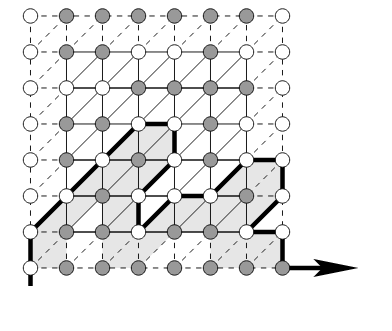
\includegraphics[scale=0.45]{HEXTHEOREM.png}
				
				\underline{Доска}
				
				Узел $(l, k) \rightarrow (\frac{l}{n}, \frac{k}{n}) \in [0, 1]^2$
				
				$0 \leq l, k \leq n$
				
				Красим узлы
				
				$v$ ~--- логический узел, $v = (v_1, v_2)$
				
				$c(v) = \min \left\{ i : \left\| f(\frac{v}{n})_i - \frac{v_i}{n} \right\| \geq \varepsilon \right\}$
			
				По лемме об игре в гексы есть одноцветная тропинка.
				
				Путь $v^0$ ~--- начальная точка тропинки, $v^N$ ~--- конечная.
				
				$v^0_1 = 0$
				
				$f(\frac{v^0}{n}) \in [0, 1]^2$, т.е. $f(\frac{v^0}{n})_1 \geq 0$
				
				$\varepsilon \leq f(\frac{v^0}{n})_1$
				
				Аналогично для $v^N_1 = 1$
				
				$f(\frac{v^N}{n})_1 \leq 1$
				
				$f(\frac{v^N}{n})_1 - \frac{v^N_1}{n} \leq -\varepsilon$
				
				$f(\frac{v^0}{n})_1 - \frac{v^0_1}{n} \geq \varepsilon$
	
				Поскольку для любых $x$ верно, что $|f(x)_1 - x_1| \geq \varepsilon$, то из этого следует, что какой-то прыжок был длиной не меньше $2 \varepsilon$, но такое невозможно, поскольку по условию если $\| x - \widehat{x} \| < \frac{1}{n} \Rightarrow \| f(x) - f(\widehat{x}) \| < \varepsilon$
				
				
	\newpage

	\section{Теорема о свойствах неопределенного интеграла}
	
		Пусть $f$, $g$ имеют первообразную на $\langle a, b \rangle$. Тогда:
		
		\begin{enumerate}
		
			\item $\int f + \int g  = \int (f + g)$
			
				$\forall \alpha \in \mathbb{R}$ $\int(\alpha f) = \alpha \int{f}$
				
			\item $\forall \varphi: \langle c, d \rangle \rightarrow \langle a, b \rangle$, $\varphi$ дифференцируема
			
				$\int f(\varphi(t))\varphi'(t)dt = F(\varphi(t)) + C$, где $F$ ~--- первообразная $f$
				
			\item $\forall \alpha, \beta \in \mathbb{R}$, $\alpha \neq 0 : \int f(\alpha x + \beta)dx = \frac{1}{\alpha} F(\alpha x + \beta) + C$
			
			\item $f$, $g$ ~--- дифференцируемы на $\langle a, b \rangle$
			
				$f' \cdot g$ имеет первообразную на $\langle a, b \rangle$
				
				Тогда $f \cdot g'$ тоже имеет первообразную и 
				
				$\int f'g = fg - \int fg'$
				
		\end{enumerate}
			
		\textbf{Доказательство}
		
		\begin{enumerate}
		
			\item $(F + G)' = f + g$
			
				$(\alpha F)' = \alpha f$
				
			\item $(F(\varphi(t)))' = f(\varphi(t))\varphi'(t)$
			
			\item $(\frac{1}{\alpha} F (\alpha x + \beta))' = f(\alpha x + \beta)$
			
			\item $(fg)' = f'g + fg'$, т.е. $fg = \int f'g + \int fg'$
			
		\end{enumerate}
\end{document}
